\documentclass{iitbthesis}
\usepackage[latin1]{inputenc}
\usepackage{amsmath}
\usepackage{amsfonts}
\usepackage{amssymb}
\usepackage{makeidx}
\usepackage{graphicx}
\usepackage{multirow}
\usepackage{epstopdf}
\usepackage{epsfig}
\usepackage{empheq}
\usepackage{hyperref}
\usepackage{bm}
\usepackage{url}
\newcommand*\widefbox[1]{\fbox{\hspace{2em}#1\hspace{2em}}}
\usepackage{appendix}
\usepackage[section]{placeins}  %to stop floating of figures b/w sections
\usepackage[a4paper, vmargin={5cm,3cm}, hmargin={3cm,2cm}]{geometry}

%%%%%%%%%%%%%%%%%%%%%%%%%%%%%%%%%%%%%%%%%%%%%%%%%%%%%
\usepackage{vmargin}
\setpapersize{A4}
\setmarginsrb{30mm}{15mm}{20mm}{22mm}{3mm}{12mm}{3mm}{10mm}
%%%%%%%%%%%%%%%%%%%%%%%%%%%%%%%%%%%%%%%%%%%%%%%%%%%%%
\setlength{\parsep}{20pt}
\setlength{\textwidth}{160mm}
\setlength{\textheight}{245mm}
\usepackage{fancyhdr}
\pagestyle{fancy}
\lhead{}
\chead{}
\rhead{\textit{Phasor Measurement Unit Development Using Low-cost Hardware}}
%\lfoot{\textit{Electrical Engineering Dept.}}
\cfoot{\thepage}
%\rfoot{\textit{IIT Bombay}}
\renewcommand{\headrulewidth}{0pt}
\renewcommand{\footrulewidth}{0pt}
\author{Rathin Dholakia}

%%%%%%%%%%%%%%%%%%%%%%%%%%%%%%%%%%%%%%%%%%%%%%%%%%%%%
\begin{document}
\thispagestyle{empty}
\begin{center}
%\vspace*{30pt}
\huge
\textbf{Thesis Title}\\
\bigskip
\bigskip
%\bigskip
%\bigskip
%\bigskip
\normalsize
\textit{Submitted in partial fulfillment of the requirements\\
                for  the degree of 
 }\\
\vspace*{0.8cm}
\textbf{MASTER OF TECHNOLOGY}\\
\textbf{(Power Electronics $ \& $ Power Systems)}\\
\vspace*{0.8cm}
\textit{by}\\
\vspace*{0.8cm}
\textbf{AUTHOR'S NAME \\(AUTHOR'S ROLL NO.)}\\
\vspace*{0.8cm}
\textit{under the guidance of}\\
\textbf{Guide's Name}\\
\vspace*{0.8cm}
\begin{figure}[h!]
 \centering
 
\includegraphics[trim=1cm 1cm 5cm 12.5cm, clip=true, width=4cm]{chapter0_initial/logo}
\end{figure}
\bigskip
\bigskip
\large
\textbf{Department of Electrical Engineering}\\
\bigskip
\textbf{INDIAN INSTITUTE OF TECHNOLOGY BOMBAY}\\
\bigskip
\textbf{June 2016}
\end{center}

\normalsize
 



% Dedication
\newpage
\thispagestyle{empty}
\vspace*{200pt}
\begin{center}
 \large

 \textit{
Dedicated to\\
\bigskip
 Whomsoever You Want To}
\end{center}
\normalsize
\chapter*{\center Dissertation Approval Certificate}
%\addcontentsline{toc}{chapter}{Abstract}

%%USING A NEW TITLE PAGE
\thispagestyle{empty}
%\vspace{0.3in}

%\hfill

%\centerline{\textbf{\large Approval Sheet}}

%\vspace{1cm}

This dissertation entitled \textbf{Thesis Title} by
\textbf{AUTHOR NAME} (Roll No: AUTHOR'S ROLL NO.) is approved for the degree of \textbf{Master of Technology} in Electrical Engineering with specialization in \textbf{Power Electronics and Power Systems} from \textbf{Indian Institute of Technology Bombay}, India.


\vspace{1.5cm}


\begin{tabular}{llc}
\hspace{4cm} & \hspace{4cm} & \hspace{1.5cm} Examiners \hspace{1.5cm} \\ \\
             &              & \hrulefill \\ \\ \\
             &              & \hrulefill \\ \\


  \hspace{1cm} Supervisor &              & Chairman   \\ \\
   \hrulefill&              &  \hrulefill \\ \\


Date:\hrulefill & & \\ \\
Place: \hrulefill & & \\
\end{tabular}


\chapter*{Declaration}
\pagenumbering{roman}
I declare that this written submission represents my ideas in my own words and where 
others' ideas or words have been included, I have adequately cited and referenced the original 
sources.  I also declare that I have adhered to all principles of academic honesty and integrity 
and   have   not   misrepresented   or   fabricated   or   falsified   any   idea/data/fact/source   in   my 
submission.  I understand that any violation of the above will be cause for disciplinary action 
by the Institute and can also evoke  penal action from the sources which have thus not been 
properly cited or from whom proper permission has not been taken when needed.

\vspace{3.0cm}
\begin{flushright}
\line(1,0){170}
\vspace*{10pt} \\
\textbf{AUTHOR NAME \\
AUTHOR's ROLL NO.}\\
Department of EE \\
IIT BOMBAY
\end{flushright}
\begin{flushleft}
-- June 2016. \textbf{CHANGE THIS}
\end{flushleft}

\pagenumbering{roman}
\chapter*{Acknowledgement}
 Write your acknowledgements here
\vspace*{30pt}
\begin{flushright}
\textbf{AUTHOR NAME}
\end{flushright}
%\chapter*{Abstract}
\singlespace
\textbf{
Write your abstract here
}
\doublespace

\tableofcontents
%\listoffigures
%\listoftables

\chapter{Introduction}
\pagenumbering{arabic}  % 1, 2, 3, 4, ...
\setcounter{page}{1}

Electric energy has become one of the most important source of energy and is widely used resource in world, with ever increasing demand of (any) resource it becomes more and more difficult to maintain the system and Power System is no exception. Power System has become a complex entity and has gone beyond the limit of manual operation and control, which makes automation and ``smart" control imperative. This creates demand for new set of measurement, operation and control tools. Out of these tools measurement tools are the most fundamental building block of the modern power system, which is now also know as "smart grid". Measurement devices are ``eyes" and ``ears" in the system to the centralized ``brain", operating-control-corrective system.  

In power system active power and frequency are the most important parameters to be monitored, flow of active power is decided by the phase angle of voltage between buses. Flow of active power decides the structure of network (transmission lines, capacity of devices etc) and hence accurate measurement of it has been of great interest since 1960-70s.\cite{agphadkebook}. Conventionally \textit{relative phase difference} between buses in the network was used, due to limitation of communication links, computational power and the economic pheasibility. This method(s) were slow, moderately accurate and dependent on a tones of heavy and/or manual calcualtion. 
After advancements in telecommunition technology and their speed \& reliability, better computation and satelite availability, trend of \textit{absolute phase difference} measurement came in to existance \cite{PMUhist}. The earliest system using absolute phase difference was reported in 1980 using LORAN-C satellite and HBG radio transmission for time reference. And during the same period Global Positioning System was being implemented by US DoD, which was immediately recognised as one of the best way of synchronising the power system, which brought the "Phasor Measurement" and "Synchrophasor" era in to existance. Lot of research was carried out and is being carried out in this area, and flurry of papers are available and are being published in different aspect of synchrophasor measurement. 
\section{Phasors, Synchrophasors and PMUs}
\subsection{Phasors: Defination}

In 1893 C. Steinmetz in his paper introduced simplified mathematcal description of a waveform of an alternating current electricity which he called as "phasor". In Physics and Engineering, \textit{phasor} is a complex number representing a sinusoidal quantity whose amplitude (A), angular velocity ($\omega$) and initial phase ($\phi$) are time-invarient.It is an analytic representation which decomposes sine function in to product of complex constants and a factor which encapsulates the frequency and time dependence. he complex constant, which encapsulates amplitude and phase dependence, is known as phasor, complex amplitude, and (in older texts) sinorx or even complexor.

Which Using Euler's formula can be represented mathematically as:
\begin{equation}\boldmath
Ae^{i(\omega t + \theta)} = A\cos(\omega t + \theta) + A\sin(\omega t + \theta)
\end{equation}

\subsection{Synchronised Phasors or Synchrophasors}
\begin{figure}
	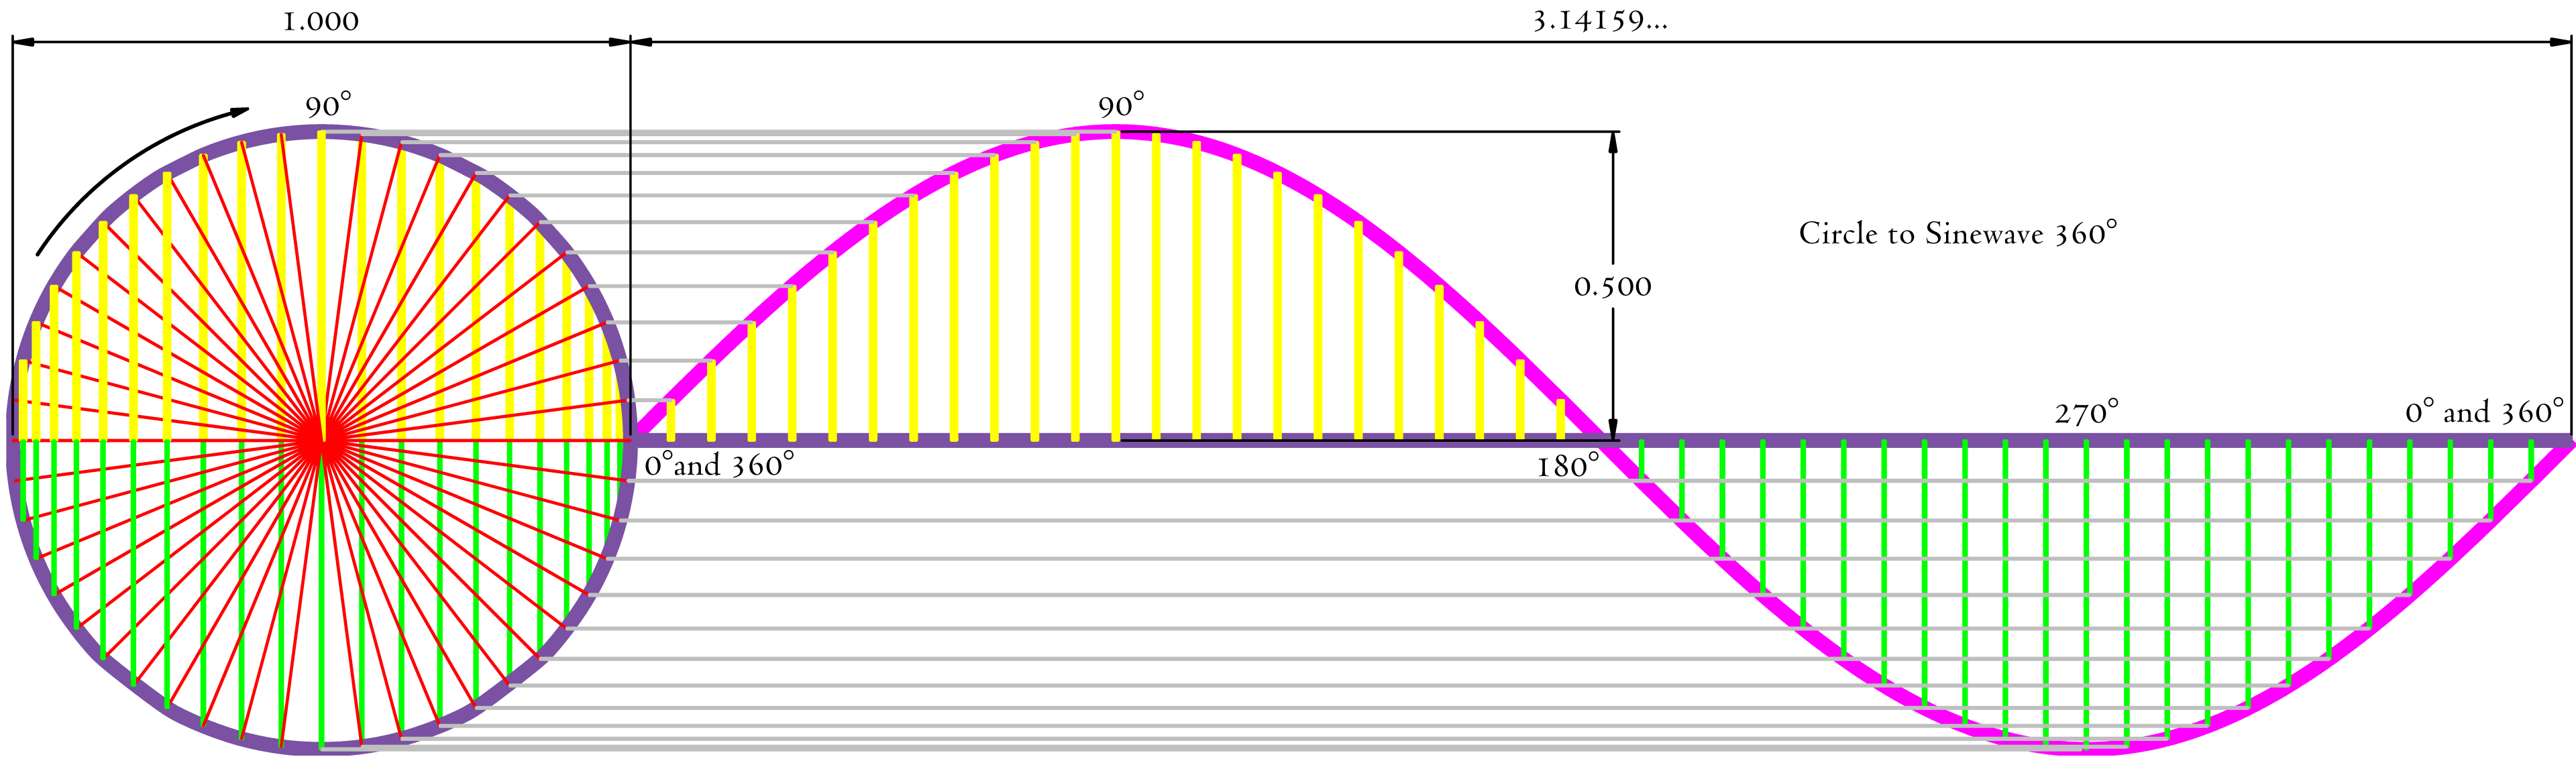
\includegraphics[width=\textwidth]{fig/Circle-To-Sine-Wave.png}
	\caption{Phasor Representation, Sampling and synchrophasor \cite{CirSinWave} .} 
	\label{fig:CirSin}
\end{figure}
 Synchronized sampling/measurement of sinusoidal complex quantity (phasor) at a precise reference (time) is called Synchronised Phasor. Time synchronization (of samples) allows synchronized real-time measurements of multiple remote location measurement points on the grid. And this resulting measurement is know as \textbf{synchrophasors} Fig. \ref{fig:CirSin}.
\subsection{Phasor Measurement Unit (PMU)}
PMU is a device which measures and estimates electrical wave in an power network using a common time source for sample synchronization. But it is important to note here that it is an ``estimate" of the phasor(!!) and not the actual measurement. 

This device was first invented by Dr. A. G. Phadke and Dr. James Thorp at Virginia Tech which is considered to be the first successful utilization of "phasors" for real-time phasors measurement that were synchronised with accurate absolute time reference provided by GPS.

\section{Wide Area Measurements}

Classically operation of grid was done by Supervisory Control And Data Acquisition(SCADA) system , which uses state estimator and other iterative solvers on system snapshot every 7-15 mins to measure and estimate the system operating point and phase angles. This approach is rather slow and less accurate but now after maturing of synchrophasor; Wide area monitoring systems (WAMS) have come in to existence, which are essentially based on the new data acquisition method of phasor estimation and allow monitoring of transmission system conditions over large areas and enable detecting and further counteracting grid instabilities. Importance and significance of synchrophasors and PMUs in WAMS can be understood when we see it from a practical perspective. Consider two geographically distant places like in India Kashmir and kaniyakumari or Aasam and Mumbai, How can we compute the phase difference of these two locations? if we want to scale the problem even further we can take American power grid where there exists Time Zone difference of 3 Hours (UTC-8.00 to UTC-5.00) from east coast to west coast, how can this be accomplished? This is where PMU and GPS comes into play, GPS enabled PMU provides an absolute time referenced \footnote{\url{http://www.physics.org/article-questions.asp?id=55}} voltage amplitude, angle and frequency (and maybe few other relevant) data of different bus to a regional control centre and eventually a central main control centre/system, this data samples are at a global reference (UTC, usually)\footnote{How accurate is GPS? know more: \url{http://www.gps.gov/systems/gps/performance/accuracy/}}. with an accuracy of few microseconds. All of this is available to the control centre at an rate of 12 to 25 snapshots per seconds, such high (and accurate) data (rate) enables system operator to operate the system efficiently and nearer to the operating limits and in case of contingencies enables them to take rapid corrective and/or preventive actions.
\begin{figure}
	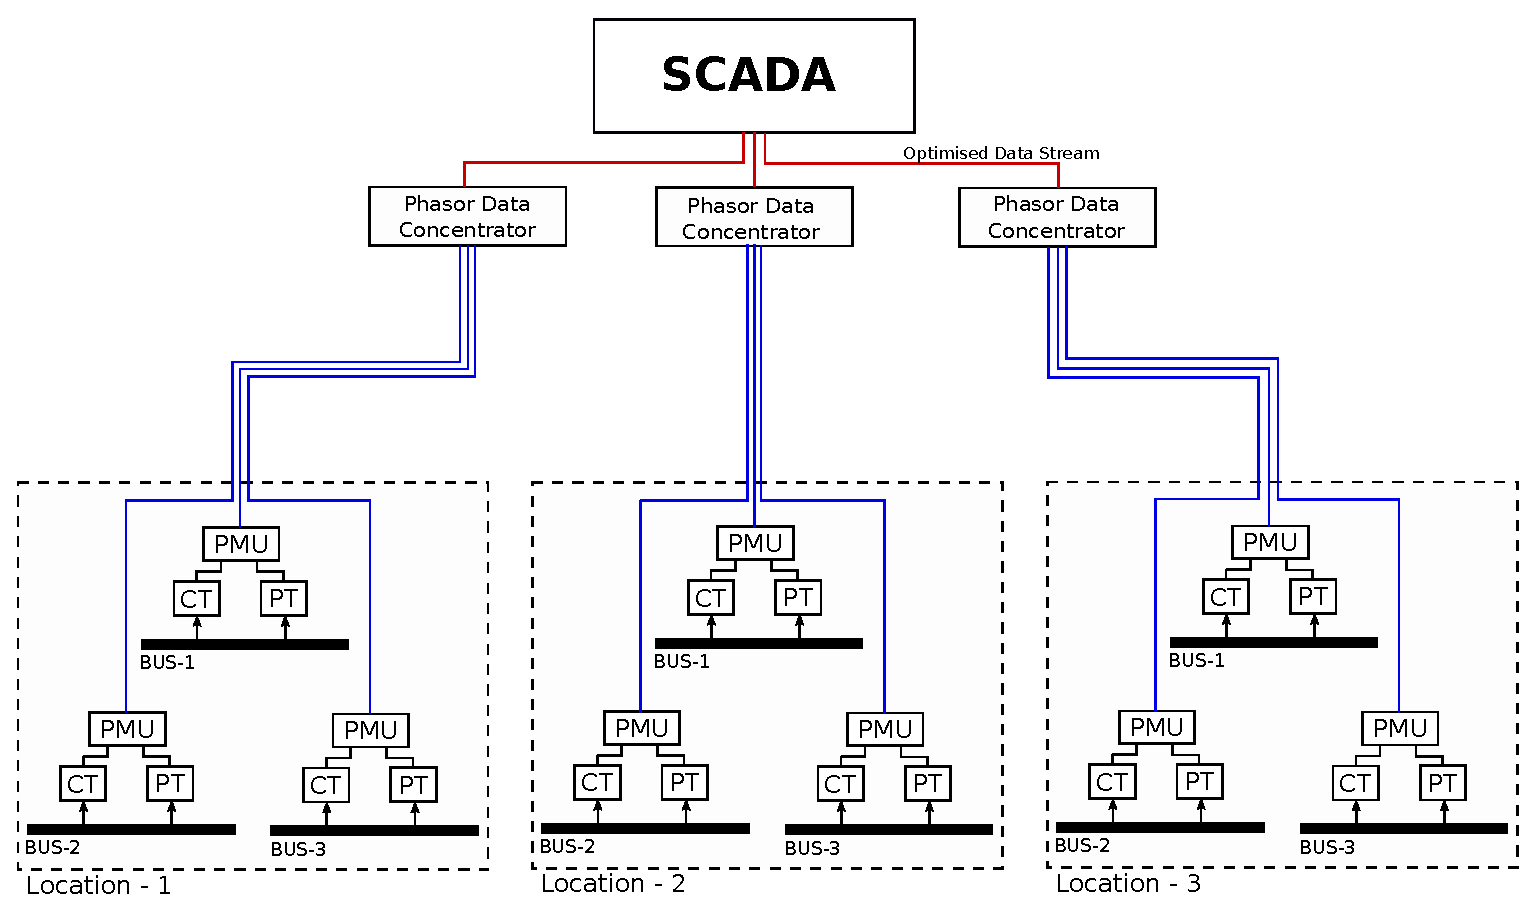
\includegraphics[width=\textwidth]{fig/wams.eps}
	\caption{Simplified structure of WAMS}
	\label{fig:wams}
\end{figure}

Fig. \ref{fig:wams} Shows a simplified architecture of modern Wide Area Measurement System. PMUs are installed at different substations on HV buses, via CTs and PTs, each PMU has multiple channels sampling AC waves at high rate. Rate of sampling varies according to the manufacturer and implementation of the scheme. Each PMU is provided a GPS receiver for accurate time with accuracy of approx 500 600 ns which is necessary for achieving time accuracy of 1-2 $\mu$s demanded by the standard. Each data after being sampled is then filtered using different DFT/FFT algorithm and is timestamped. This time stamped data is then sent to either SCADA or to a local Phasor Data Concentrator, which consolidates the data stream coming from different PMUs and send an bandwidth optimized data stream to the higher PDC or SCADA. 

\section{IEEE C37.118 Standard}

\subsection{Need of the standard}
This standard is for synchrophasor measurement, it defines synchronised phasor and frequency measurement is substation alng with requirements for measurement verification. Role of this standard is that measurements taken complient with and abiding to this standard will be readily accurately usable for power system analysis purposes. Standard achieves this by stating minimum necessary performance requirements of time-tagging, sampling and communication requirements to which a PMU has to adhere.

IEEE 1344-1995 is the original standard which was succeeded by IEEE C37.118-2005. 2005 standard mostly followed equipment manufacturers and the system integrators and was stating performance of steady-state conditions. After the advancements and development in fault analysis dynamic synchrophasors were being used for the control and analysis.  which was the major reason of Revision-2011, which was immediately followed by revision 2014 which simplified the stringent norms laid down by it's predecessor.

\subsection{Definations, acronyms and abbriviations}

Before diving in to details lets clear out few useful terminologies for ease of understanding and appreciation of the subject:\\
\textbf{Phasor:} A complex equivalent of a sinusoidal wave quantity such that the complex modulus is the cosine wave amplitude, and the complex angle (in polar form) is the cosine wave phase angle.\\
\textbf{UTC:} Its is the time of day at the earth's prime meridian.\\
\textbf{ROCOF:} It is the measure at which the frequency changes in a given instance of time.\\
\textbf{Rate of change of Frequency Error (RFE):} The measure of error between the theoretical ROCOF and the measured ROCOF for the given instant of time.\\
\textbf{Frame:} A data frame or a frame of data is a set of synchrophasor, frequency, and ROCOF measurements that corresponds to the same time stamp.\\
\textbf{Anti-aliasing:}The process of filtering a signal before sampling to remove components of that signal whose frequency is equal to or greater than the Nyquist frequency (one-half the sample rate). If not removed, these signal components would appear as a lower frequency component (an alias).\\
\textbf{Nyquist frequency:} A frequency that is one-half the sampling frequency of a discrete signal processing
system.\\

\subsection{Requirements and Compliance}
Just like all other engineering devices PMU's reliability, accuracy  and precision are very crucial for its application and hence different kinds of test are done to validate its performance. Hence just like other measuring devices PMU standards are defined which states minimum performance requirement(s). All device should at least meet the requirement stated by the standards, according their application.


\subsubsection{Total Vector Error}
Classically error is the deviation of the measurement from the ideal quantity. It is computed from the difference between the Actual to the measured value. In case of synchrophasors the comparison involves difference in both amplitude and angle which are time dependent making the task even tougher. these quantities are considered combinely in the standards and is called "Total Vector Error (TVE)" \cite{c37.118}.  

TVE is an expression of the difference between a ``perfect" sample of a theoretical synchrophasor and the estimate given by the unit under test at the same instant of time. The value is normalized and expressed in per unit of the theoretical phasor. Which can be mathematically represented as: 
\begin{equation}
TVE(n) = \sqrt{\frac{ (\hat{X}_r(n) - X_r(n))^2 + (\hat{X}_i(n)-X_i(n))^2} {X_r(n)^2 + X_i(n)^2}}
\end{equation}
Here $ \hat{X}_r (n)$ and $\hat{X}_i(n) $ are the estimated values of the given phasor and $X_r$ and $X_i$ are the theoretical values.
To be complient with standard, PMU shall provide synchrophasor, frequency, and ROCOF measurements that meet the requirements as per the standards at a given time instance \textit{n}. Similarly for freq and ROCOF the validation will be done using following equations:
\begin{eqnarray}
FE == |f_{true}-f_{measured}| = |\Delta f_{true}-\Delta f_{measured}| \\
RFE == |(df/dt)_{true}-(df/dt)_{measured} |
\end{eqnarray}

\subsubsection{Class of PMU:}
Depending up on the application PMU are classified in two types and depending upon the class their error tolerance is evaluated, there are two classes:
\begin{enumerate}
	\item \textbf{Measurement Class (M):} As the name suggests these are used for measurement and instrumentation purposes. These PMUs are intended for slower response time and greater precision. These kind of PMUs are used for analytical purposes and hence often do not require minimal (reporting) delay or fastest reporting speed.
	\item \textbf{Protection Class (P):} These PMUs are designed for fastest responses time. They may have (slightly) inferior reporting precision and soft-realtime operation. 
	mandates no explicit filtering
\end{enumerate} 

\subsubsection{Validation \& Testing }

To get the TVE, compliance tests are performed and during the test only the quantity under test is varied from the reference condition as per the test and other relevant quantities are maintained at reference condition. There are following kind of compliance tests:
\begin{enumerate}
	\item Steady-state compliance
	\begin{enumerate}
		\item Steady-state synchrophasor measurement requirements
		\item Steady-state frequency and ROCOF measurement requirements
	\end{enumerate}
	\item Dynamic compliance
	\begin{enumerate}
		\item Synchrophasor measurement bandwidth requirements using modulated test signals
		\item Ramp of system frequency
		\item Step changes in phase and magnitude
	\end{enumerate}
\end{enumerate} 
The TVE tolerance for each case wont be mentioned here as those tables can be looked into the standards.


\subsubsection{Time Synchronization}

The PMU should be capable of receiving time from a reliable and accurate source such as GPS that can provide time traceable to UTC with sufficient accuracy for calculating Total Vector Error (TVE), Frequency Error and rate of change of frequency error (RFE), all measurements are synchronized to UTC.
This is a vital parameter because time error of 1$\mu$s would result in to 0.022 degree and 0.018 degree in 60 Hz and 50 Hz systems respectively. And a phase error of 0.57$\deg$ will result in to 1\% TVE. This corresponds to error tolerance of $\pm26 ~\mu$s for 60 Hz and $\pm 31 ~\mu s$ for 50 Hz system.

\subsubsection{Reporting Rate}
Estimate of synchrophasor, Frequency and ROCOF will be made so that they can be reported to data concentrator and the reporting rate should be constant i.e. the time difference between two reports received from a PMU should be same. This reporting rate will be integer number of times per second and should be in integer multiple of the of the power nominal-frequency. Hence required rate of reporting as mentioned below:

\begin{table}
	\begin{center}
		\setlength\arrayrulewidth{1pt}
		\begin{tabular}{|c|c|c|c|c|c|c|c|c|c|}
			\hline
			System Frequency & \multicolumn{3}{c}{50 Hz} & \multicolumn{6}{|c|}{60 Hz}\\
			\hline 
			Reporting Rate (Fs)& 10 & 25 & 50 & 	10& 12 &15 & 20 & 30 & 60\\
			\hline
		\end{tabular}
	\end{center}
\end{table}
 

\subsubsection{Performance Parameters}
These are the parameters considered as qualitative factors to judge the PMU performance. 

\begin{itemize}
	\item  \textit{Measurement response time:} Measurement response time is the time to transition between two steady-state measurements before and
	after a step change is applied to the input. This is measured by applying a step change in amplitude or phase and holding the input constant otherwise and measuring the time taken  by the PMU to settle to a steady-state value. response time is determined from the accuracy evaluation of the measurements, not step time or the stepped	parameters themselves.
	\item \textit{Measurement delay time:} It is the time difference between the step input applied and the measurement time that the output reaches 50\% of the final or steady state value.  
	\item \textit{Measurement Reporting Latency:} Reporting Latency is the time lag between the event occurs in the power system and it is reported in the data. It is one of the important quantitative and qualitative parameter, as it depends on al most all factors involved like sample window, filter delay, processing time, processor speed etc. Here reporting rate and PMU class play major role in deciding the delay. 
	\item \textit{Measurement and operational errors:} It is a self-health-test flag. as per standard PMU should send a status flag with each measurement stating the error at PMU end. this error bit can incorporate issue in any aspect(s) like ADC error, memory over flow, etc.
\end{itemize}

\subsubsection{Communication Compliance}

\chapter{Implementation}
\section{Requirements and Goals}
Depending upon the function we can split the design of a PMU in three parts. 
A. Signal Input \& Sampling part
B. Processing of Samples  
C. Transmission of data
Different parts will havediffern
\subsection{Subsection 1}
\section{Chapter 2 Section 2}

\chapter{Results and Discussion}
The device has been designed completely from scratch. So to make it standard compliant it is necessary to test it's all aspect and keep them well below the limit so that final results are well within the stipulated guideline. Hence, here qualitative and quantitative results are presented which include computation latency, reporting rate \& variation, ADC response(s) and amplitude \& frequency estimation.

\subsubsection{Computation delay}
The following graph show the delay distribution of DFT computation, left hand side of plot shows normal operation while right hand side of the plot shows a loaded system performance. The "on-load" condition wont occur in real-life scenario but this was done just to evaluate overall capability and performance.
\begin{figure}[h]
	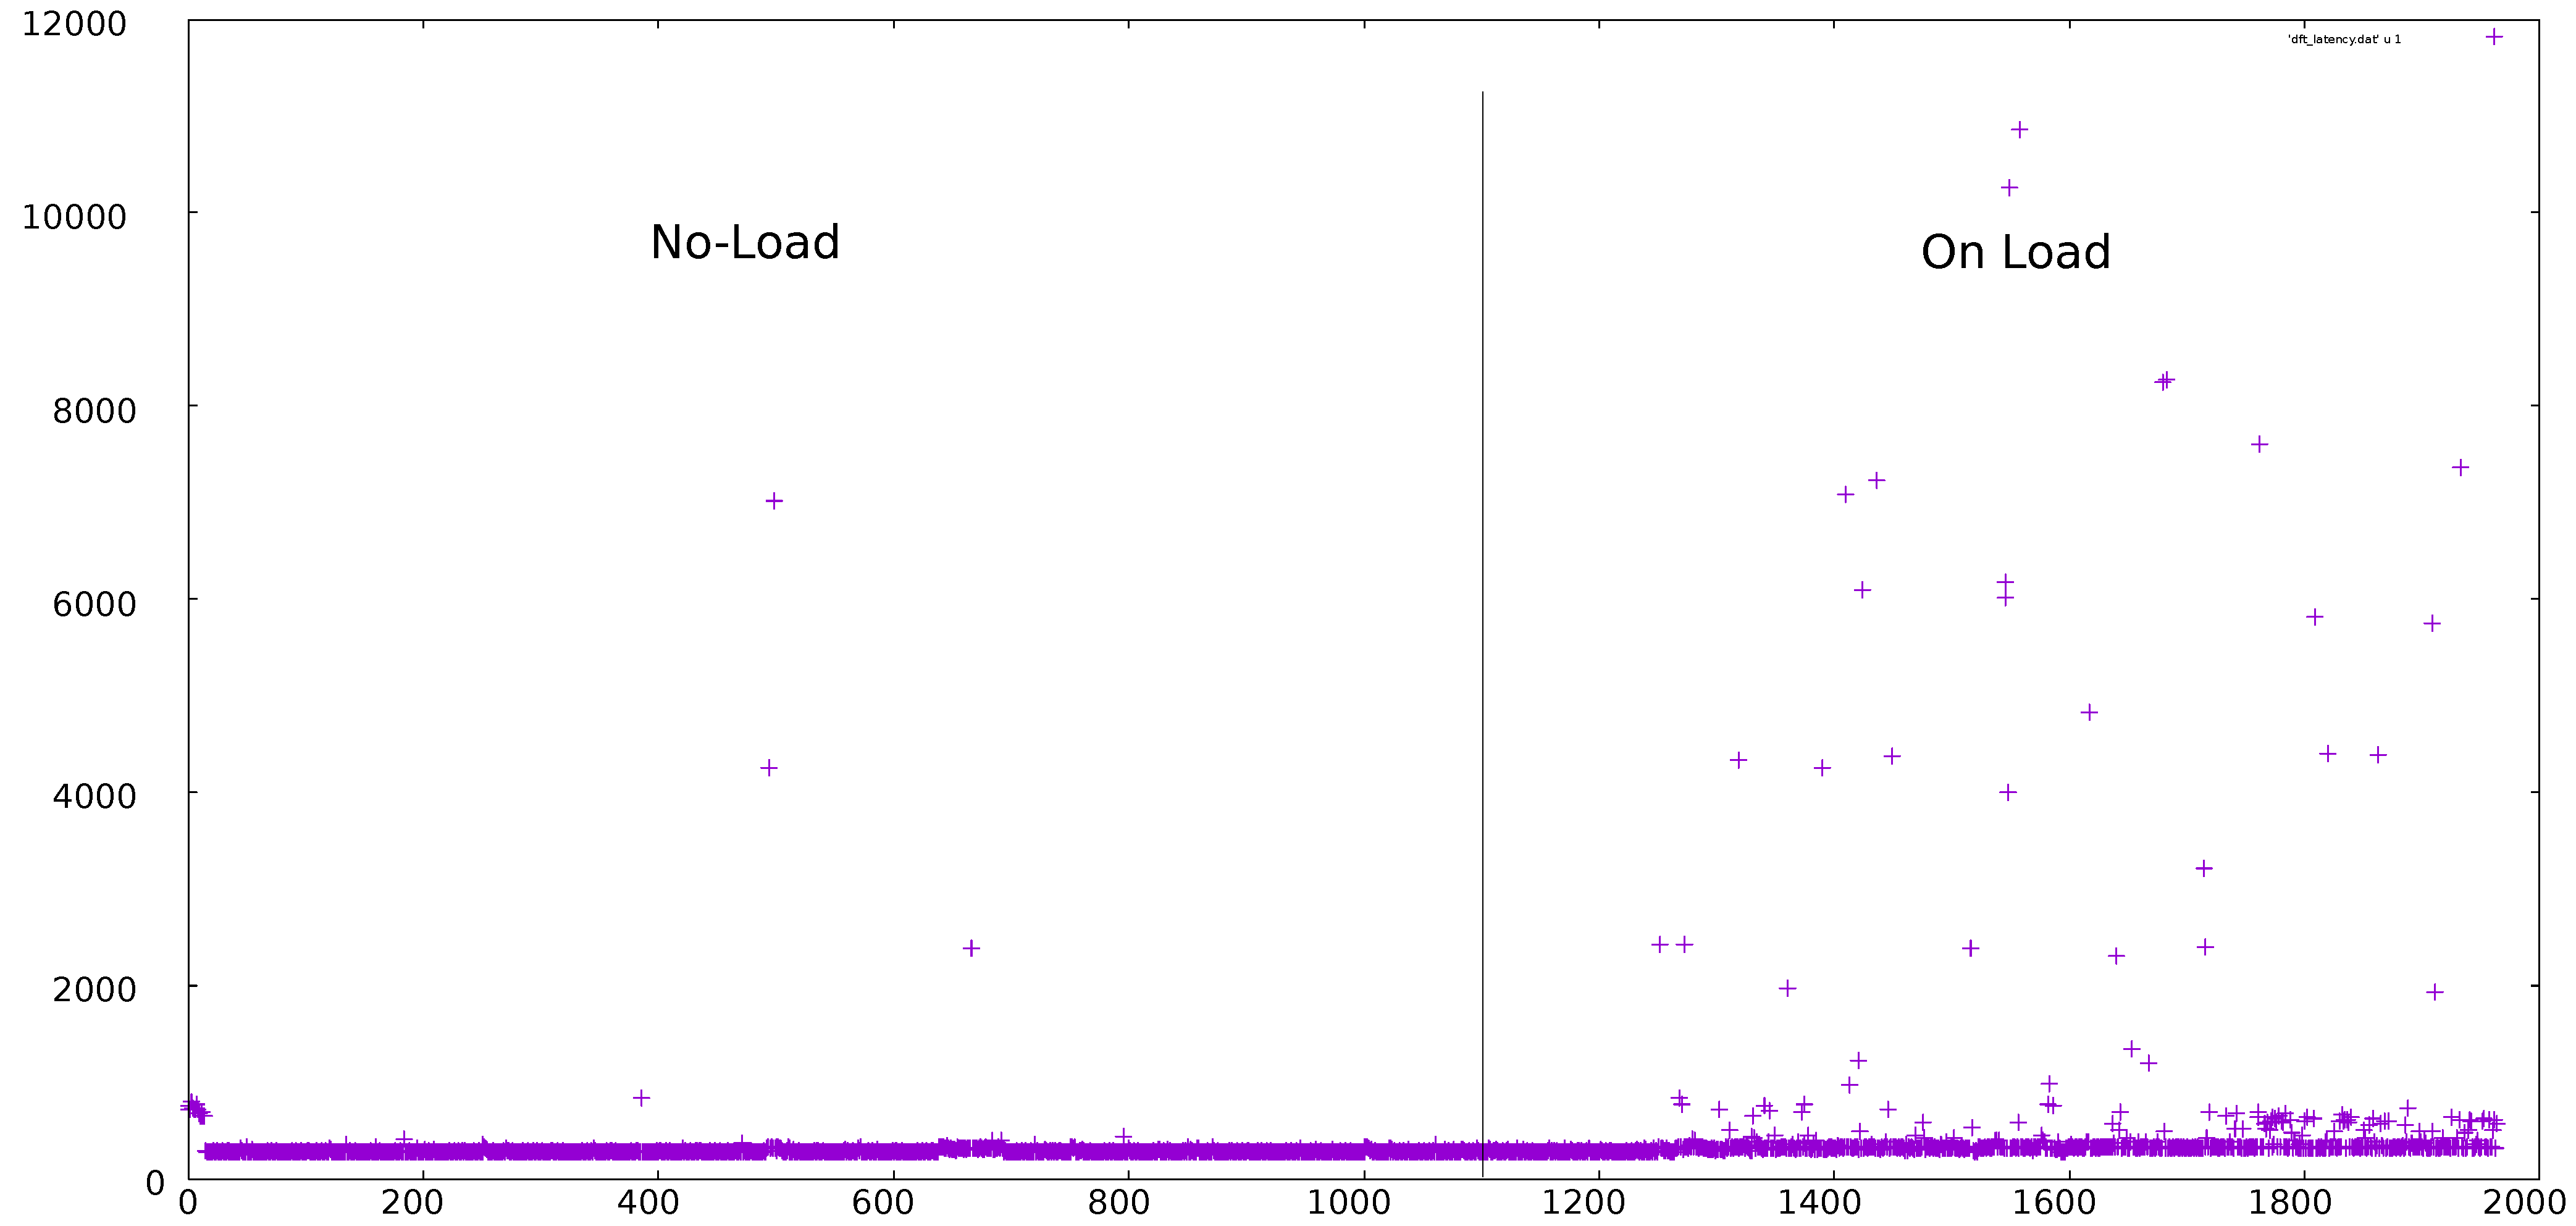
\includegraphics[scale=0.23]{fig/delay_test.eps}
\end{figure}

%\chapter{Conclusion}

\section{Chapter 4 Section 1}
\subsection{Subsection 1}
\section{Chapter 4 Section 2}

\begin{appendix}
%=======================================================
\chapter{OMAP-L137 implementation}
Initially OMPA-L137 EVM was used to develop PMU. And considerable development was done but during a testing it got damaged and started malfunctioning. So, a brief description is given here about what all things were done and it's concept.

 OMAP-L137 EVM doesn't have Analog to Digital Converter on board hence an interfacing circuit is designed. While designing the ADC board following criteria were considered.
\begin{itemize}
	\item Good sampling rate: ~200 kSamples/Sec
	\item Minimum no of channels: 3 + 3 = 6 (3 - $\phi$ voltage and current) 
	\item Interfacing type: It should be memory addressable and voltage level compatible  to the EVM.
	\item Input type: FSS analog output is differential which can be configured as single ended and its voltage level is $\pm$10V
\end{itemize}
  
On the basis of above stated requirements several chips were filtered for the application and finally AD7864 was chosen. AD7864 is a high speed 4 channel simultaneous (dedicated) sampling successive approximation ADC with \textit{bi-polar input} having conversion time as low as $1.65 \mu s$. Chip's sampling rate can go as high as 500 ksps \cite{uguide:adc}. Chip's conversion sequence can be controlled through hardware as well as software, its default operating voltage of control and data pins is 5v but it has a special output voltage level shifter for interfacing it with 3.3v processors and controllers. A variant of the chip AD7864-1 was chosen as our ADC due to it's direct input voltage compatibility range of $\pm$ 10 V. This ADCs are fairly advance and hence they have been interfaced with a special asynchronous peripheral interfacing architecture called Extended Memory InterFace (EMIF-A), which is exclusively available in OMAP-L13x series processors.

 Extended Memory InterFace (EMIF) has two parts A \& B out of which EMIF-B is having \textit{Enhanced Direct Memory Access} controller (EDMA3) which enables the processor for multi-threaded rapid memory access and hence it is exclusively for highspeed SDRAM interfacing where as interface \textit{A} (EMIF-A) is developed for generic purposes, it's further details are given below:

\subsubsection{EMIF-A}
EMIF-A controller is a 16-bit databus based versatile controller \cite{uguide:emifa}, designed to interact with variety of devices like 
\begin{itemize}
	\item Single Data Rate (SDR) RAM
	\item Asynchronous devices like NAND \& NOR flash memory and SRAM
\end{itemize}

\begin{figure}[h]
	\centering
	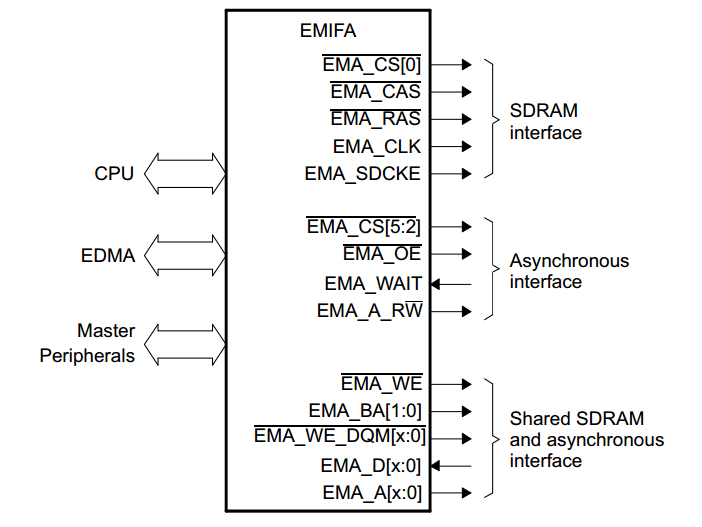
\includegraphics[scale=0.4]{fig/EMIFA.png}
	\caption{EMIFA Block Diagram \cite{uguide:emifa} }
	\label{fig:EMIFA}
\end{figure}

It contains lot of features to ease and facilitate the usage of asynchronous devices. A functional block diagram is given here in Fig: \ref{fig:EMIFA} It is apparent from Fig: \ref{fig:EMIFA}, that it has 4 chip selects and, read and write for them and 16 data channels. which makes it very convenient for interfacing multiple peripherals at a time. 


\begin{figure}[ht]
	\centering
	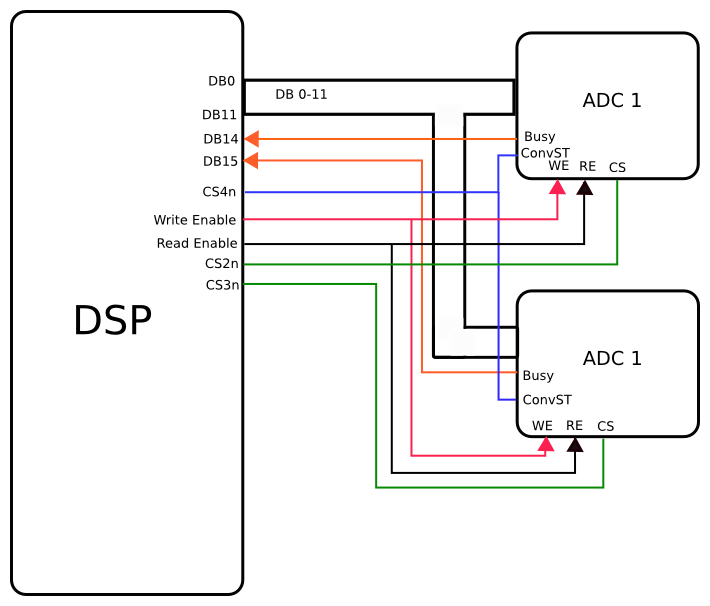
\includegraphics[scale=0.4]{fig/ADC_board.png}
	\caption{ADC Board block diagram}
	\label{fig:adc_board}
\end{figure}
Using the EMIF-A and the AD7864-1 a ADC board was designed for interfacing OMAP-L137 with Full Spectrum Simulator. Above Fig: \ref{fig:adc_board} shows the design logic of that ADC board. 


\subsubsection{ADC board Logic}
Due to EMIFA, interfacing of ADC board became quiet convenient rather than using pins in GPIO mode. So the logical flow of the board is as follows:

\begin{itemize}
	\item 6 input channels are required hence 2 ICs are used
	\item Chip Select (CS), Read, Write, and databits from 0 - 11 are directly available from the EMIFA interface, and they are shared with both the chips.
	\item AD7864 has sequence selection which has been configured through hardware, and Clock source has been kept internal. because of this both the pins \texttt{INT/EXT\_CLK} \& \texttt{H/S select}
	\item AD7864 has 3 control output \texttt{Busy}, \texttt{FIRSTDATA} and \texttt{EOC}. Out of these only \texttt{busy} is observed via a data line (data bits 16 \& 15). Data is \textbf{and}ed is not read until data line 15 \& 14 are not zero.
	\item AD7864 supports two kinds of data reading 1) Reading during the conversion 2)Reading after the conversion. Here we are going to use \textit{Reading After the conversion}, below is the timing diagram of the chip for understanding the proper functioning of the circuit.
\end{itemize}


\begin{figure}[h]
	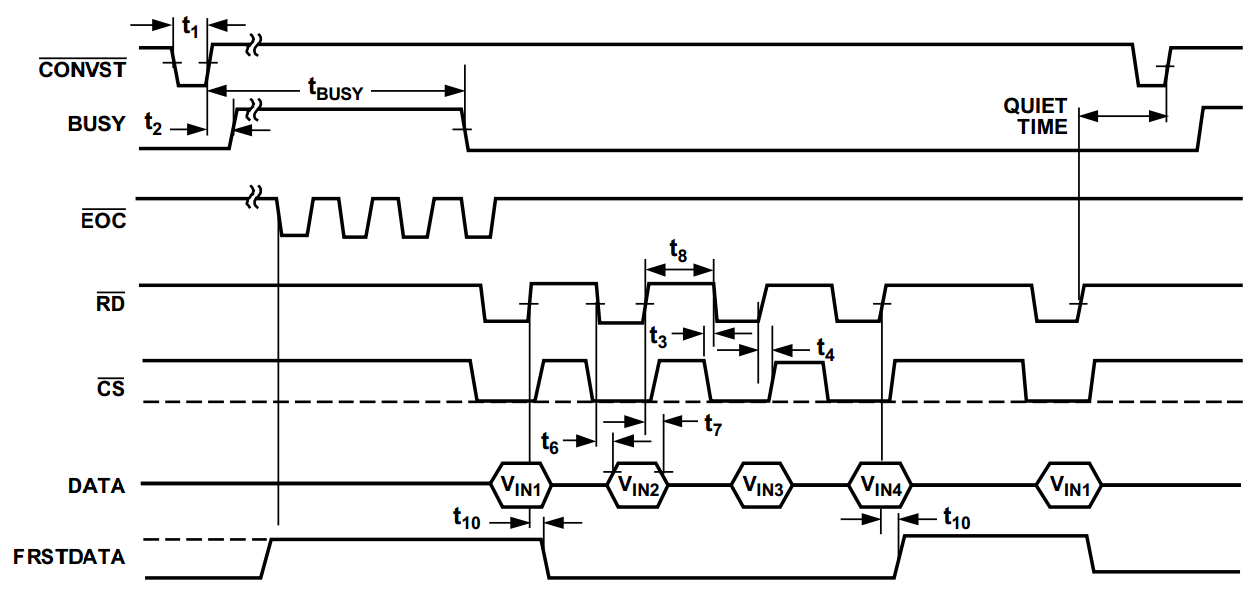
\includegraphics[width =\columnwidth]{fig/adc_time_diag.png}
	\caption{ADC Reading After the Conversion timing \cite{uguide:adc}}
	\label{fig:adc_timing}
\end{figure}
Now we will see the operation that takes place when sampling  is to be done:
\begin{itemize}
	\item Assert start of conversion (\texttt{CONVST}) is asserted via \texttt{EMA\_CS(4)}
	\item Due to this chip will start the conversion processes which will make \texttt{BUSY} high,
	\item Status of \texttt{BUSY}  will be checked via \texttt{DB15} \& \texttt{DB14} pins of the EMIFA header, for both the chips untill they are \texttt{low} again.
	\item The moment \texttt{BUSY} goes low, \texttt{EMA\_CS[2]} and \texttt{EMA\_A\_RE} are asserted with which AD7864 starts putting data on data lines. this processes of asserting is repeated for 4 times, for each channel. The same is done using \texttt{EMA\_CS[3]} for getting data from 2nd ADC chip.
\end{itemize}
Apart from ADC board another important component in PMU is GPS signal. A NavSynch CW-12TIM GPS receiver is will be interfaced. The receiver provides three type of output signal.
\begin{itemize}
	\item 1PPS - Synchronized with the start of the UTC second
	\item 10MHz FOUT - The maximum time interval error (MTIE) of this signal is 4us at the interval of 446.8 Ks.
	\item UART - Data communication port for UTC data and other control/status information
\end{itemize}
The receiver has an on board RTC which maintains the time information in loss of satellite fix.

\subsubsection{Software Implementation}
OMAP-L137 being a dual core asymmetric type processor it will run two instance of OSes or program, (i) DSP side and (ii) ARM side.  

\begin{itemize}
	\item \textbf{DSP Side:}
	DSP can be programmed in 2 ways (a) Boiler plate programming (b) Using an OS. Boiler plate programming would be the fastest running implementation yet an challenging task to accomplish as all the necessary device drivers and interfacing has to be done manually. In case of OS based implementation, an abstraction layer is there which will have all the necessary device drivers already available, user just has to use the library and write a higher level C/C++ code. Though second approach lucrative, a compromise needs to be made in regards to the latency. Due to existence of a kernel and a scheduler would give you relatively less fast execution. In our device, our timing requirements were not very intensive and could have been met easily hence OS was use.
	
	Taxas Instruments, provides two OS options (a) DSP/BIOS (b) SYS/BIOS, DSP/BIOS being less flexible and slower as well as getting obsolete and phased out by TI, Sys/BIOS was chosen. Sys/BIOS provides preemptive multi-threading, hardware abstraction, real-time analysis, and configuration tools.The libraries are optimized for execution time and majority of them are written in assembly	language. The threading model provides threads for interrupts and tasks. Priorities and blocking characteristics of these can be easily controlled. For the application, all Sys/BIOS objects are configured statically and bound into a single image
	
	\item \textbf{ARM Side:} On the ARM side by default MontaVista OS was provided along with EVM. For our purpose, real-time micro kernel OS-- QNX RTOS was chosen. Officially QNX-6.4 is supported but QNX- 6.5 source can be modified to work on OMAP-L137. Few salient feature of QNX are 
	\begin{itemize}
		\item Micro kernel: Runs most of the functions as tasks which can be easily disabled reducing the size of memory footprint. The kernel is basically just a scheduler which allows smaller OS ticks to be handled efficiently. The PMU application requires features like the TCP/IP stack, I/O handlers, Timers and Memory Management. Rest of the overheads like filesystem, DMA, RTC, USB can been stripped out.
		\item TCP/IP stack: QNX has TCP/IP stack which is tiny has very optimised yet with all features.
		\item  Multitasking: Two primary task run on ARM side, One is to acquire Time data word from GPS and update the system time and to send data packets over ethernet.
	\end{itemize}

\end{itemize}
It is very important to keep the memory footprint low as both the OSes use the same RAM and it has only 64 MB RAM, which is also being used for data storing.

\subsubsection{Implementation}
Strategy of implementation is as follows:
\begin{enumerate}
	\item Low level tasks of controlling ADC and sensing 1PPS will be done by DSP core.  Start of conversion, data ready and read will be asserted by DSP core. 
	\item Data received from the ADC upon which DFT computation will be performed and data will be passed to ARM via shared memory.
	\item ARM core running QNX will read the results from shared Memory and data packet will be formed which will be sent to the PDC.
	\item QNX will also communicate with GPS module to receive and decode time status word over UART. Time information will be used in time tagging the data before being sent over the network. 
\end{enumerate}
Before the board got damaged following things were implemented already implemented on it:
\begin{itemize}
	\item DSP core Timer was configured to assert start of conversion signal to ADC chip
	\item GPS 1 PPS signal was interfaced with one of the data pin EMIF-A, which was configured as GPIO, which was generating interrupt. 
	\item Testing of data read function was being carried out.
\end{itemize}

\chapter{Compiler Optimisation}

There are several compilation time and run time optimization available with GCC suit which can really impact the performance of a program \cite{compilerOpti}. These options control various sorts of optimizations. Without any optimization option, the compiler's goal is to reduce the cost of compilation and to make debugging produce the expected results. Turning on optimization flags makes the compiler attempt to improve the performance and/or code size at the expense of compilation time and possibly the ability to debug the program. There are 4 major levels of optimization defaults, that are provided by GCC. which are -O, -O1, -O2, -O3.
\begin{enumerate}
	\item \textbf{-O O1}
	Optimize. Optimizing compilation takes somewhat more time, and a lot more memory for a large function. With -O, the compiler tries to reduce code size and execution time, without performing any optimizations that take a great deal of compilation time.
	
	\item \textbf{-O2} Optimize even more. GCC performs nearly all supported optimizations that do not involve a space-speed tradeoff. The compiler does not perform loop unrolling or function inlining when you specify -O2. As compared to -O, this option increases both compilation time and the performance of the generated code.
	
	\item \textbf{-O3} Optimize yet more. -O3 turns on all optimizations specified by -O2.  
\end{enumerate}

Level \texttt{-O3} was used for optimizing the code for this project and \texttt{O3} is the highest level of optimization possible by GCC. The list of flag passed by O3 are listed below:


 



\begin{table}[h]
	\centering

	\caption{Compiler Optimization Flags}
	\label{my-label}
	\textit{
	\begin{tabular}{|l|l|}
		\hline
-ffast-math & -floop-optimize   \\ \hline
-fdefer-pop  & -foptimize-sibling-calls   \\ \hline
 -fdelayed-branch & -fguess-branch-probability \\ \hline 
-fthread-jumps & -fcse-follow-jumps  -fcse-skip-blocks   \\ \hline
-fmerge-constants & -frerun-cse-after-loop  -frerun-loop-opt  \\ \hline
-fstrength-reduce		& -fgcse   -fgcse-lm   -fgcse-sm \\ \hline
 -fdelete-null-pointer-checks 		&  -fcaller-saves\\ \hline
-fregmove 		& -fexpensive-optimizations \\ \hline
-fsched-interblock -fsched-spec	&  -fschedule-insns -fschedule-insns2 \\ \hline
-fstrict-aliasing &  -freorder-blocks  -freorder-functions \\ \hline
-fpeephole2		& -falign-functions  -falign-jumps \\ \hline
-falign-loops  -falign-labels		&  -fcrossjumping \\ \hline
-fif-conversion & -fif-conversion2 \\ \hline
 -fcprop-registers & -fforce-mem \\ \hline
	\end{tabular}
}
\end{table}

More detailed description of each flag can be found on this GCC C compiler \texttt{man} pages \cite{compilerOpti}.

It worth while to note here that becomes almost impossible to debug the code once \textbf{O3} level optimization is applied as all the frames and pointers and data section are realigned and all runtime level checks are removed to increase the performance. So it is necessary that code is compiled, tested and debugged in normal compilation process and after it is stable only the final executable be generated with these codes.

\subsubsection{$NEON ^{\circledR}$ Vectorization }
Since cortex A8 processors ARM has incorporated a Neon block and VFP accelerator. Neon is a SIMD (Single Instruction Multiple Data) accelerator processor integrated in as part of the ARM Cortex-A8, what it means is that  during the execution of one instruction the same operation will occur on up to 16 data sets in parallel, it is also synonymous with the term vector processor. Since there is parallelism inside the Neon, you can get more MIPS or FLOPS out of Neon than you can a standard SISD processor running at the same clock rate:

  Apart from compiler optimization Neon vectorization is also used here to optimized the speed and boost the performance of the code. Vectorization results in to as big as \~1000 $\mu$s. To achieve vectorization, three ways are there, (1) Compiler option (2) Neon intrinsics (3) Assembly code. In our case to insert the Neon initialization code, compiler option is used. Which won't results in to fastest implementation yet can achieve considerable speed boost.


\chapter{C37.118 Frame Structure}


\begin{figure}[h]
	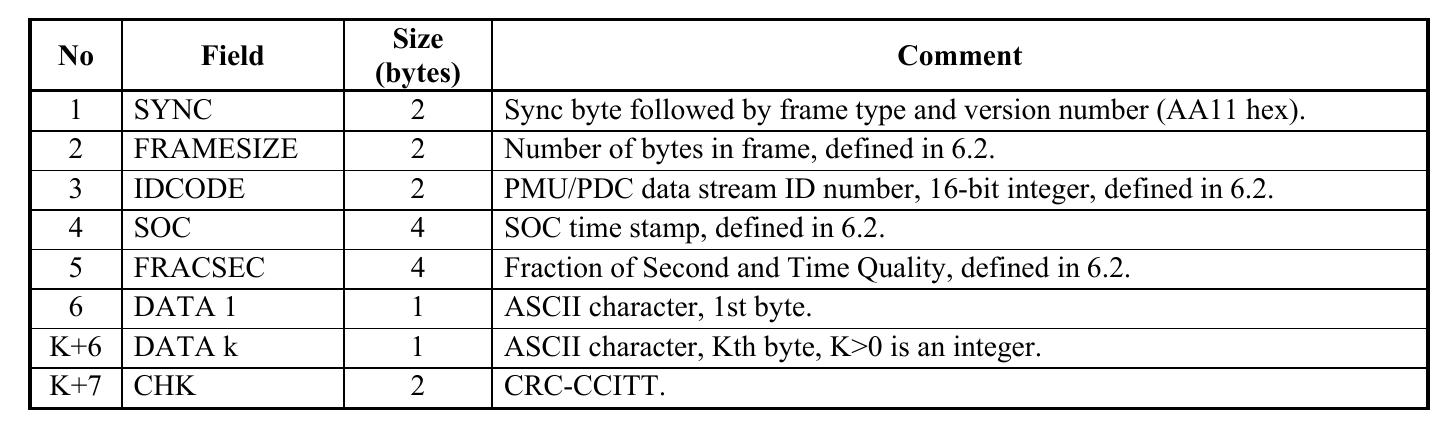
\includegraphics[width=\textwidth]{fig/hdr_frame.png}
	\caption{Header Frame structure \cite{c37.118.2}}
\end{figure}

\begin{figure}[h]
	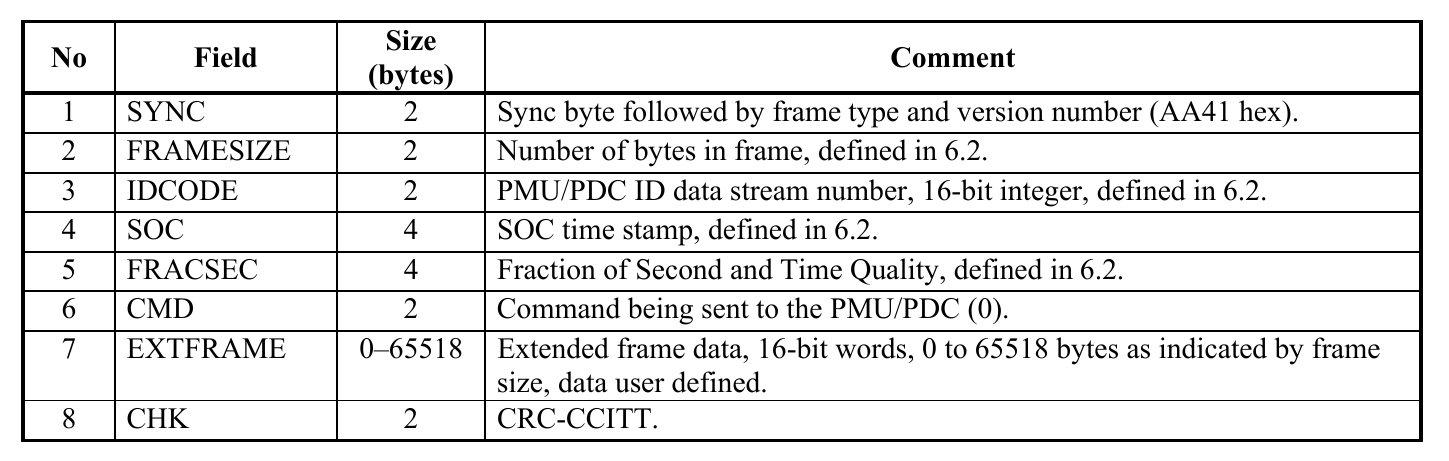
\includegraphics[width=\textwidth]{fig/cmd_frame.png}
	\caption{Command Frame structure \cite{c37.118.2}}
\end{figure}

\begin{figure}[h]
	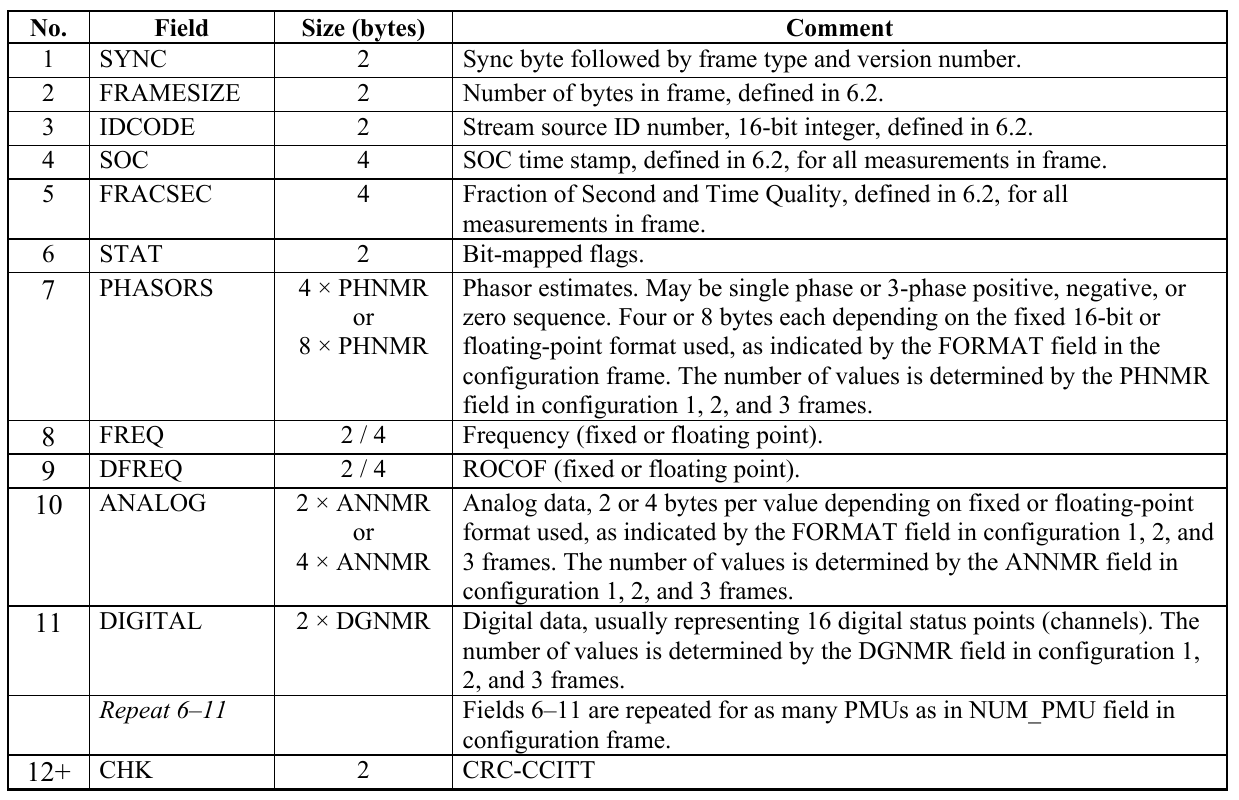
\includegraphics[width=\textwidth]{fig/data_frame.png}
	\caption{Data Frame Structure \cite{c37.118.2} }
\end{figure} 


\begin{figure}[h]
	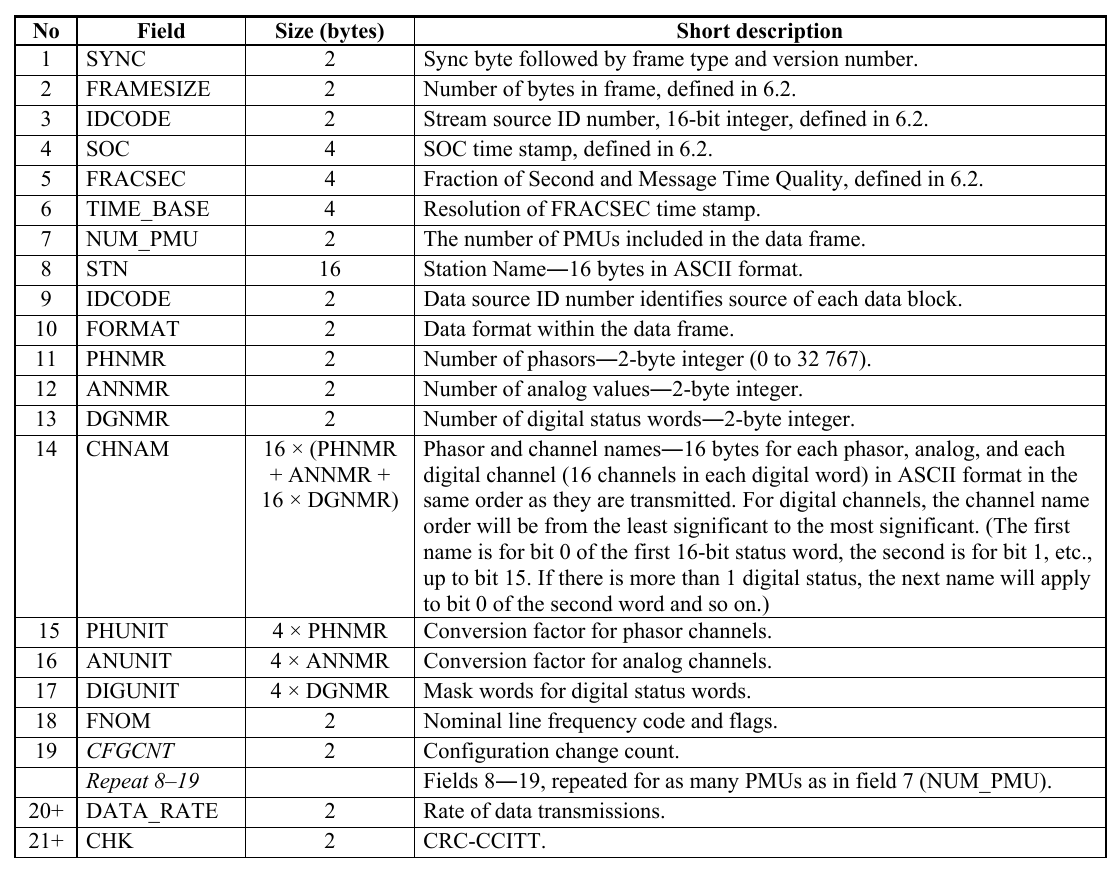
\includegraphics[width=\textwidth]{fig/cfg_frame12.png}
	\caption{Configuration Frame 1 - 2 Structure \cite{c37.118.2}}
	\label{fig:cfg_12}
\end{figure} 

Following configurations shown in Fig:\ref{fig:cfg_12} and in Fig: \ref{fig:cfg_3} are machine readable messages communicated before the data frame is sent. They are the full description of device status and capability, here only brief details are given, further details can be read from the standards- C37.118.2   
\begin{figure}[h]
	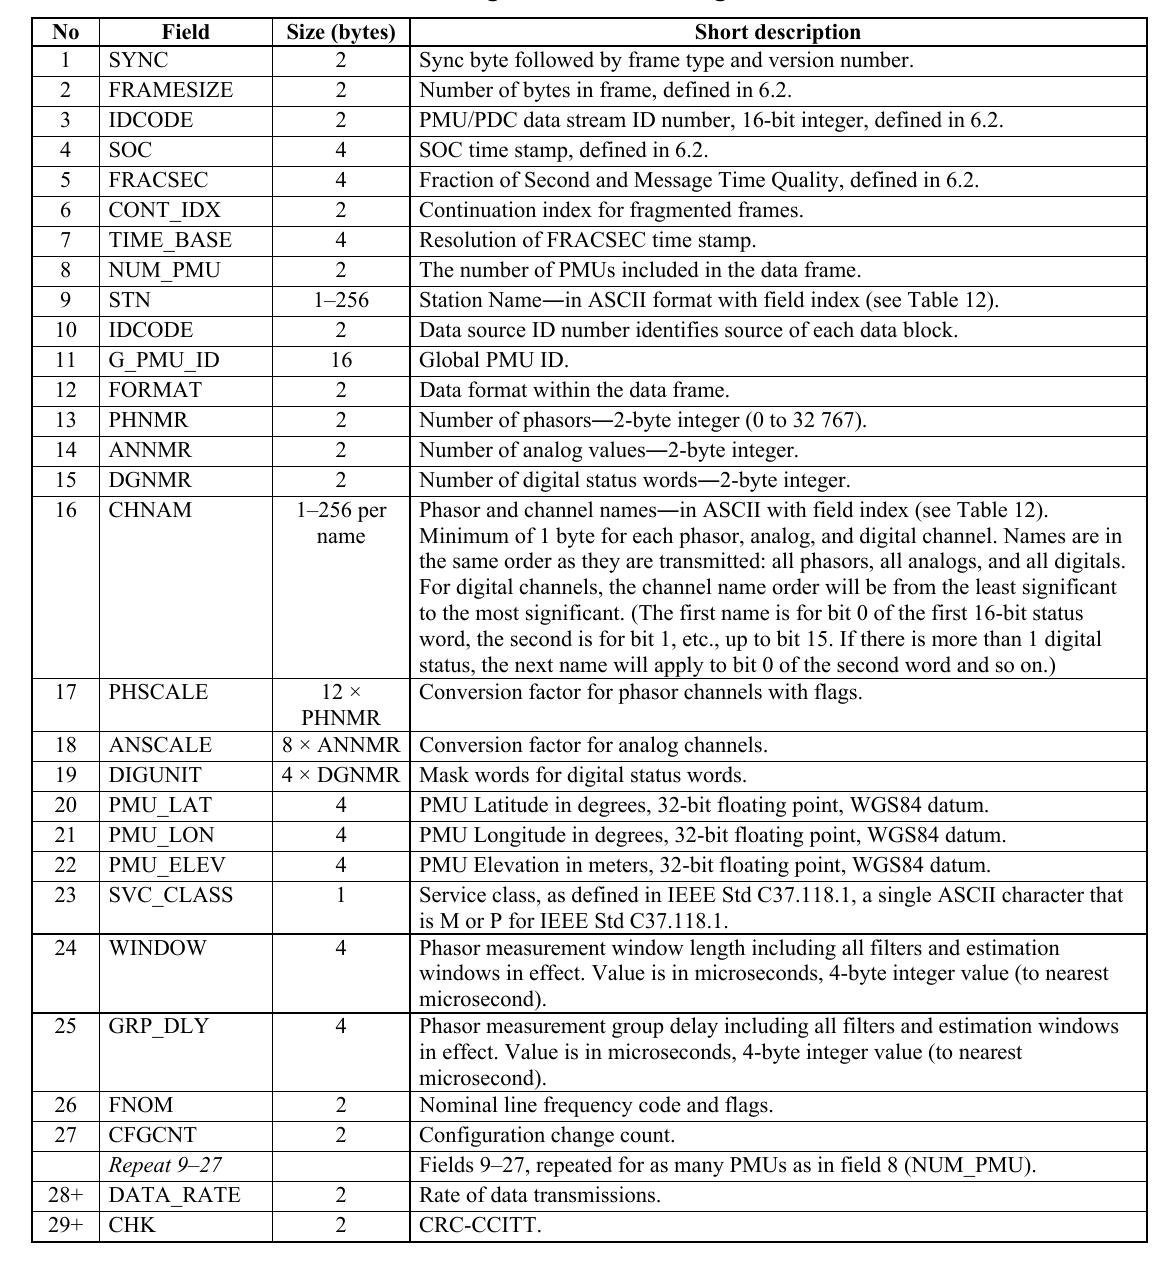
\includegraphics[width=\textwidth]{fig/cfg_frame3.png}
	\caption{Configuration Frame 3 Structure \cite{c37.118.2}}
	\label{fig:cfg_3}
\end{figure} 


\end{appendix}


\bibliographystyle{IEEEtran}
\bibliography{reference1}
                                                                                                                 
\end{document}
